\documentclass{article}

\PassOptionsToPackage{numbers,compress}{natbib}
\usepackage[dblblindworkshop]{neurips_2026}
\workshoptitle{On-Device Intelligence: Foundation Models under Real-World Constraints}

\usepackage[utf8]{inputenc}
\usepackage[T1]{fontenc}
\usepackage[hidelinks]{hyperref}
\usepackage{microtype}
\usepackage{graphicx}
\usepackage{booktabs}
\usepackage{amsmath,amssymb}
\usepackage{xcolor}
\usepackage{url}
\usepackage{placeins}

\newcommand{\pcross}[1]{P_{\mathrm{cross},#1}}
\newcommand{\synops}{\mathrm{SynOps}}

\title{Parameter Scope Matters:\\
MNE-L2 for Reliable Low-Latency ANN-to-SNN Conversion}

\author{Anonymous Authors}

\begin{document}

\maketitle

\begin{abstract}
Spiking neural networks (SNNs) use sparse, discrete spike events to support event-driven and potentially energy-efficient inference on neuromorphic hardware. ANN-to-SNN conversion offers a practical route to deep SNNs by reusing well-trained ANN parameters, thereby avoiding the difficulty of training deep SNNs directly. However, thresholded spike representations can be fragile under noise. To investigate how source training shapes this robustness, we study the parameter scope of regularization and identify a failure: applying L2 to batch-normalization (BN) affine parameters can make converted SNNs substantially less robust than applying it only to weights. We analyze this failure through local spike-count boundary crossings and propose margin-normalized effective L2 (MNE-L2), which rescales the L2 penalty on source weights by BN-folded amplification relative to each layer's conversion margin. Across five-seed CIFAR experiments, MNE-L2 improves high-noise accuracy over all-parameter L2 by up to $62.06$ percentage points while reducing clean firing activity and estimated arithmetic energy. These findings expose regularization scope as an important training choice and demonstrate that MNE-L2 improves the reliability--efficiency trade-off for low-latency SNN inference.
\end{abstract}

\section{Introduction}

Spiking neural networks (SNNs) communicate through discrete spike events rather than dense activations, enabling sparse, event-driven computation and potentially energy-efficient inference on neuromorphic hardware~\cite{davies2018loihi}. Realizing these advantages with deep models, however, requires accurate inference within a short simulation horizon. High-accuracy deep SNNs can be obtained either by direct training or by converting artificial neural networks (ANNs). ANN-to-SNN conversion is particularly practical because it reuses well-trained ANN parameters and avoids the difficulty of optimizing deep SNNs directly~\cite{rueckauer2017conversion,sengupta2019going}. Converted SNNs often require many simulation steps to approximate ANN activations. Reducing the timestep budget lowers latency and event cost but increases finite-time conversion error~\cite{bu2022optimal}. Recent conversion and calibration methods have substantially improved low-timestep accuracy~\cite{hu2023fast,bu2022optimal}, making reliability under deployment noise increasingly important.

Because SNN inference is built from thresholded spike events, perturbations can abruptly alter spike counts and propagate through later layers. Prior work has studied noise sensitivity in trained SNNs and adversarial robustness after conversion~\cite{ding2024robust,ozdenizci2024adversarially}. Most low-latency conversion methods, however, focus on reducing clean conversion error through activation design, calibration, or membrane-potential correction. How the source ANN's training choices shape post-conversion robustness has received much less attention.

To fill this gap, we start with a controlled ablation of L2 regularization, a standard source-ANN training choice whose parameter scope is often left implicit. In networks with batch normalization (BN)~\cite{ioffe2015batch}, an L2 penalty can cover weights alone or also the BN affine parameters. Figure~\ref{fig:bn-scope} compares weights-only L2 with penalties that additionally include BN-$\beta$, BN-$\gamma$, or both. Including BN-$\gamma$ causes a sharp accuracy collapse even when moderate Gaussian noise ($\sigma=1$) is applied independently at each SNN timestep, whereas weights-only L2 and weights plus BN-$\beta$ remain stable. This scope-dependent failure motivates our stability analysis.

\begin{figure}[h]
  \centering
  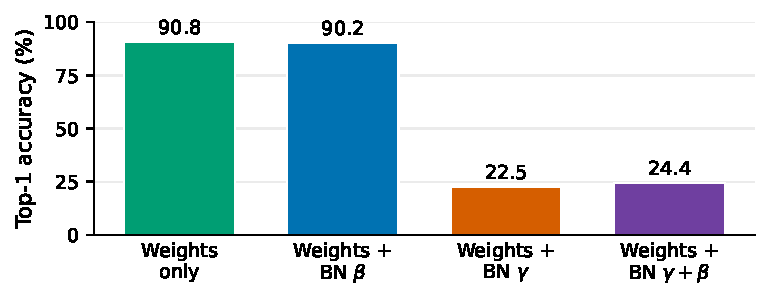
\includegraphics[width=0.68\textwidth]{images/bn_affine_scope.pdf}
  \caption{CIFAR-10 VGG16 parameter-scope ablation with Gaussian noise applied independently at each SNN timestep. At $\sigma=1$, including BN-$\gamma$, with or without BN-$\beta$, causes a sharp accuracy collapse.}
  \label{fig:bn-scope}
\end{figure}

To explain this scope-dependent failure, we analyze how additive perturbations cross local spike-count boundaries as they propagate through a converted network. Local risk is governed by effective noise relative to the nearest transition margin: downstream BN-folded weights determine perturbation amplification, while the following integrate-and-fire (IF) threshold sets the nominal conversion margin. Guided by this analysis, we propose margin-normalized effective L2 (MNE-L2). It rescales L2 updates on convolutional and linear weights so that layers with larger folded amplification relative to their margin receive stronger regularization, while BN affine parameters and IF thresholds receive no gradient from the regularization term.

Our contributions are:
\begin{itemize}
    \item We identify an underexplored L2 parameter-scope failure and isolate BN-$\gamma$ as the affine term that distinguishes the unstable settings in a controlled four-way ablation.
    \item We derive a local boundary-crossing analysis that relates conversion margin and perturbation amplification to the stability of discrete spike counts.
    \item We show across CIFAR VGG13/16/19 and ImageNet ResNet-18 that MNE-L2 substantially improves high-noise accuracy over all-parameter L2 and, on CIFAR, reduces firing density and estimated arithmetic energy.
\end{itemize}

\section{Related Work}

\paragraph{Low-latency ANN-to-SNN conversion.}
Early ANN-to-SNN conversion methods rely on weight normalization, threshold balancing, and activation normalization~\cite{diehl2015fast,rueckauer2017conversion}. At short simulation horizons, finite-time mismatch has been reduced through optimized potential initialization~\cite{bu2022optimized}, parameter calibration~\cite{li2021free}, residual-membrane-potential and offset-spike correction~\cite{hao2023reducing,hao2023bridging}, mitigation of temporal misalignment with probabilistic spiking neurons~\cite{bojkovic2025temporal}, and quantization-aware ANN training~\cite{hu2023fast,bu2022optimal}. SpikeConverter reduces the activation-to-spike representation gap through specialized conversion dynamics~\cite{liu2022spikeconverter}, while more recent methods learn explicit conversion-error compensation or bridge quantized activations and spiking neurons~\cite{liu2025efficient,yang2025neubridge}. Collectively, these methods improve clean conversion accuracy or latency by modifying activation design, calibration, or conversion dynamics. In contrast, we retain QCFS as a fixed conversion backbone and study how source-weight regularization affects post-conversion robustness.

\paragraph{Regularization scope in normalized networks.}
Normalization can make preceding weights scale-invariant, causing L2 regularization to act through parameter scale and the effective learning rate rather than solely as a conventional capacity penalty~\cite{van2017l2}. Practical CNN training recipes often restrict weight decay to convolutional and fully connected weights while excluding biases and BN affine parameters~\cite{he2019bag}. More generally, whether BN-$\gamma$ should be regularized depends on its architectural role, and practices vary across libraries and implementations~\cite{kim2024guidelines}. These studies concern ANN optimization and clean-task performance. We instead study how regularization scope shapes internal-noise stability after conversion; MNE-L2 scales source-weight regularization by BN-folded amplification relative to the boundary margin of the following IF activation.

\paragraph{Stability and noise sensitivity.}
Perturbation stability has been studied through Lyapunov bounds for ANNs~\cite{rahnama2020robust} and membrane-potential dynamics in trained SNNs~\cite{ding2024robust}. Related work has also analyzed average input-noise stability and Fourier-spectrum concentration in wide LIF-SNN classifiers~\cite{araya2026random}, as well as classifier-level adversarial robustness after conversion~\cite{ozdenizci2024adversarially}. We instead derive a neuron-level upper bound on the probability that internal Gaussian noise crosses a spike-count boundary in a converted SNN. This local analysis motivates MNE-L2 rather than a worst-case classifier-robustness objective.

\section{Method}

\subsection{Low-latency QCFS conversion}

We first describe the quantization clip-floor-shift (QCFS) conversion used in our experiments and then derive the proposed regularizer. For activation $x$, threshold $\lambda$, and quantization level $L$, the source ANN uses~\cite{bu2022optimal}
\begin{equation}
q_L(x;\lambda)=\frac{\lambda}{L}
\left\lfloor L\,\mathrm{clip}\!\left(\frac{x}{\lambda},0,1\right)+\frac{1}{2}\right\rfloor .
\label{eq:qcfs}
\end{equation}
At inference, an integrate-and-fire (IF) layer emits a length-$T$ spike sequence whose rate represents the quantized activation.

\subsection{Local noise-to-margin analysis}

Let $z$ be the clean output of an IF layer and $\tilde z=z+\epsilon$, where $\epsilon\sim\mathcal{N}(0,\sigma^2 I)$. Let $\mathcal{B}_l$ contain the QCFS boundaries of layer $l$ and $d_l(u)=\min_{b\in\mathcal{B}_l}|u-b|$. Under a local additive model $\delta_l\sim\mathcal{N}(0,\sigma_{\mathrm{eff},l}^2)$, changing the quantization bin requires crossing a boundary, so
\begin{equation}
\Pr[q_L(u+\delta_l)\neq q_L(u)\mid u]
\leq 2\,\mathrm{Q}\!\left(\frac{d_l(u)}{\sigma_{\mathrm{eff},l}}\right),
\label{eq:crossing-bound}
\end{equation}
where $\mathrm{Q}$ is the Gaussian upper-tail function. In an idealized aggregation of $C$ independent inputs over $T$ timesteps, $\sigma_{\mathrm{eff}}^2\leq\sigma^2M/(CT)$ when $M$ bounds the mean squared weight. The nominal QCFS half-cell margin is $h_L=\lambda/(2L)$, giving
\begin{equation}
\rho_{\mathrm{nom}}=\frac{h_L}{\sigma_{\mathrm{eff}}}
\geq \frac{\lambda\sqrt{CT}}{2L\sigma\sqrt{M}}.
\label{eq:nominal-stability}
\end{equation}
Thus stability improves with aggregation over width and time but decreases as conversion cells become finer. This local scaling law is not a network-level accuracy guarantee; its assumptions and post-hoc layerwise diagnostics are given in Appendices~\ref{app:local-model} and~\ref{app:layerwise}.

\subsection{Margin-aware weight regularization}

Equation~\eqref{eq:nominal-stability} suggests controlling perturbation amplification relative to the following conversion margin. For each convolution or linear layer followed by BN and an IF activation, we therefore fold the BN scale into the matched weight while stopping the regularization gradient through BN and the IF threshold:
\begin{equation}
\widetilde W_{l,o}=
\operatorname{sg}\!\left(\frac{\gamma_{l,o}}{\sqrt{v_{l,o}+\epsilon_{\mathrm{BN}}}}\right)W_{l,o},
\qquad
M_{\mathrm{eff},l}=\frac{1}{C_l}\sum_o\|\widetilde W_{l,o}\|_F^2.
\label{eq:effective-weight}
\end{equation}
Using $M_{\mathrm{eff},l}$ as a proxy for the layer's BN-folded amplification, the trainable layer-dependent factor in the inverse squared nominal stability is $L_l^2M_{\mathrm{eff},l}/\lambda_l^2$, up to the fixed aggregation and injected-noise terms. We use this factor to weight L2 without requiring clean--noisy paired forward passes during training:
\begin{equation}
\mathcal{R}_{\mathrm{MNE}}=
\sum_l\frac{L_l^2 M_{\mathrm{eff},l}}
{\operatorname{sg}(\lambda_l)^2+\varepsilon},
\label{eq:mne}
\end{equation}
where $\operatorname{sg}$ denotes stop-gradient. The source objective is $\mathcal{L}_{\mathrm{task}}+\eta\mathcal{R}_{\mathrm{MNE}}$, with coefficient $\eta$ specified in the appendix. Layers without a following IF threshold are excluded. MNE-L2 does not optimize the margin directly; it uses the current margin and BN-folded amplification to scale the L2 gradient on $W_l$, applying stronger weight regularization where the amplification-to-margin ratio is larger. BN-$\gamma$, BN-$\beta$, and $\lambda_l$ receive no gradient from this term. Thus, all-parameter, weights-only, and selective L2 penalties are different interventions even when their coefficients are numerically similar.

\section{Experiments}

\subsection{Setup}

We evaluate QCFS VGG16 on CIFAR-10/100~\cite{krizhevsky2009learning} and QCFS ResNet-18 on ImageNet~\cite{deng2009imagenet,he2016deep}. Unless noted, $L=T=16$ and rate-uniform IF inference first aggregates the full $T$-step input and then distributes output spikes uniformly, suppressing unevenness error. At every timestep, zero-mean Gaussian noise is sampled independently and added to the feature map after the input IF. L2-all regularizes all trainable parameters, whereas L2-wo and L1-wo regularize only convolutional and linear weights. CIFAR results report mean $\pm$ sample standard deviation over five seeds; ImageNet and the scope ablation are single-seed, with one perturbation stream shared across the scope settings. Hyperparameters are fixed before noise evaluation without clean-accuracy matching; full protocols appear in the appendix.

\subsection{BN gain distinguishes the unstable scope settings}

Figure~\ref{fig:bn-scope} gives the $\sigma=1$ snapshot, while Figure~\ref{fig:bn-scope-sweep} shows the full scope sweep. Weights-only L2 and weights plus BN-$\beta$ retain $75.63\%$ and $70.65\%$ at $\sigma=3$; both settings containing BN-$\gamma$ reach chance by $\sigma\approx1.5$. Their near-overlap implicates gain, rather than bias, as the principal scope difference in this controlled run.

\begin{figure}[h]
  \centering
  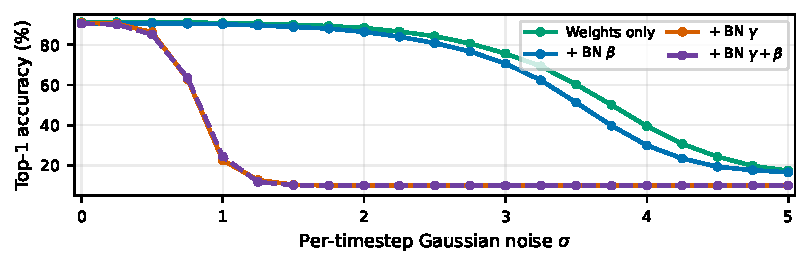
\includegraphics[width=0.82\textwidth]{images/bn_affine_scope_sweep.pdf}
  \caption{Full single-seed CIFAR-10 VGG16 parameter-scope sweep. Each point uses the same stored perturbation stream for the four scope settings.}
  \label{fig:bn-scope-sweep}
\end{figure}

Post-hoc layerwise diagnostics show that settings containing BN-$\gamma$ develop lower margin-to-noise ratios and higher crossing rates in late blocks, whereas weights-only L2 and MNE-L2 remain more stable (Appendix~\ref{app:layerwise}); this single-seed intervention does not establish a universal BN mechanism, but shows why ``L2'' should report its parameter scope.

\subsection{MNE-L2 across CIFAR and ImageNet}

Figure~\ref{fig:robustness-benchmarks}(a,b) extends the stress test to five independently trained seeds per CIFAR dataset. At $\sigma=5$, MNE-L2 reaches $72.06\%$ on CIFAR-10 and $41.14\%$ on CIFAR-100, versus $39.40\%$ and $17.91\%$ for weights-only L1; all-parameter L2 collapses near $\sigma=1$. The ordering persists for VGG13/19 (Appendix~\ref{app:depth-transfer}). On the single ImageNet checkpoint, MNE-L2 retains $33.07\%$ at $\sigma=1$, versus $21.11\%$ for L1-wo, and remains highest at $\sigma=2$ (Figure~\ref{fig:robustness-benchmarks}(c)).

\begin{figure*}[t]
  \centering
  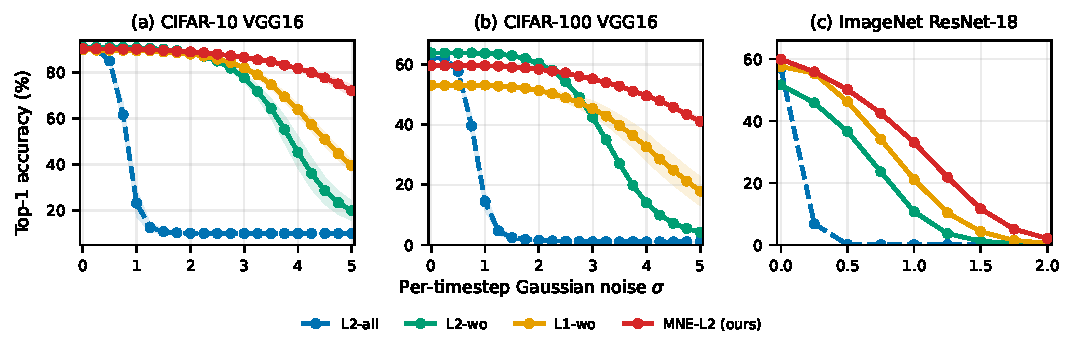
\includegraphics[width=\textwidth]{images/cifar_imagenet_absolute_noise.pdf}
  \caption{Per-timestep Gaussian-noise sweeps at $L=T=16$. (a,b) CIFAR VGG16 curves are five-seed means; bands show sample standard deviations across the five seeds. (c) ImageNet ResNet-18 uses a single-seed checkpoint and therefore has no uncertainty band. MNE-L2 is highlighted in red and all data points use circular markers.}
  \label{fig:robustness-benchmarks}
\end{figure*}

\subsection{Clean sparsity, robustness, and estimated energy}

\begin{table*}[t]
\caption{Five-seed CIFAR VGG16 robustness--activity summary at $T=16$ (mean $\pm$ sample standard deviation; 10,000 test images per seed). Accuracy is measured under per-timestep Gaussian noise at $\sigma=5$; firing density and arithmetic energy use clean inference. The best value in each dataset and metric is bold, and the second-best is underlined. Clean accuracy and full activity distributions appear in Appendix~\ref{app:cifar-tables}.}
\label{tab:cifar-deployment-main}
\centering
\scriptsize
\setlength{\tabcolsep}{4.5pt}
\begin{tabular}{llrrr}
\toprule
Dataset & Method & Clean firing density & Clean energy (mJ) & Acc. at $\sigma=5$ (\%) \\
\midrule
CIFAR-10  & L2-all & $0.105\pm0.003$ & $0.585\pm0.006$ & $10.00\pm0.00$ \\
          & L2-wo  & $0.102\pm0.001$ & $0.505\pm0.003$ & $19.92\pm4.29$ \\
          & L1-wo  & $\mathbf{0.077\pm0.001}$ & $\mathbf{0.402\pm0.005}$ & $\underline{39.40\pm2.60}$ \\
          & MNE-L2 (ours) & $\underline{0.083\pm0.001}$ & $\underline{0.472\pm0.003}$ & $\mathbf{72.06\pm2.57}$ \\
\midrule
CIFAR-100 & L2-all & $0.106\pm0.003$ & $0.558\pm0.008$ & $1.05\pm0.06$ \\
          & L2-wo  & $0.105\pm0.001$ & $0.522\pm0.002$ & $4.21\pm0.24$ \\
          & L1-wo  & $\mathbf{0.084\pm0.002}$ & $\mathbf{0.429\pm0.005}$ & $\underline{17.91\pm4.84}$ \\
          & MNE-L2 (ours) & $\underline{0.090\pm0.001}$ & $\underline{0.494\pm0.004}$ & $\mathbf{41.14\pm1.23}$ \\
\bottomrule
\end{tabular}
\end{table*}

Table~\ref{tab:cifar-deployment-main} compares all four regularizers at high noise. On CIFAR-10, MNE-L2 lowers clean firing from $0.105$ to $0.083$ and energy from $0.585$ to $0.472$ mJ relative to L2-all, while retaining $72.06\%$ rather than $10.00\%$ accuracy at $\sigma=5$. The same robustness ordering holds on CIFAR-100, where MNE-L2 reaches $41.14\%$ and L2-all reaches $1.05\%$. L1-wo is the sparsest and least energy-intensive method, but Appendix~\ref{app:cifar-tables} shows that it trails MNE-L2 by $6.49$ clean CIFAR-100 points.

Following Horowitz~\cite{horowitz2014computing}, estimated energy charges repeated first-layer MACs at $4.6$ pJ and clean event-triggered ACs thereafter at $0.9$ pJ (Appendix Eq.~\ref{eq:energy}). Noisy firing is excluded because injected events would confound deployment cost. The estimates omit memory, neuron updates, control, interconnect, and leakage, and are not device measurements.
\FloatBarrier

\section{Discussion and Conclusion}

Regularization scope materially affects robustness after ANN-to-SNN conversion. Under our post-input-IF Gaussian-noise protocol, settings that regularize BN-$\gamma$ exhibit stronger late-layer instability, while MNE-L2 scales source-weight regularization by BN-folded amplification relative to the following IF margin. Across the tested CIFAR models, MNE-L2 improves high-noise accuracy and reduces firing activity and estimated arithmetic energy. Because energy is estimated from arithmetic counts rather than measured on neuromorphic hardware, the efficiency gains require device-level validation. These results motivate explicit reporting of regularization scope and evaluating robustness alongside clean conversion accuracy.

\clearpage
\bibliographystyle{unsrtnat}
\bibliography{reference}

\appendix

\section{A Local Precision--Width--Time Model}
\label{app:local-model}

Consider an idealized normalized aggregation of independent perturbations,
\begin{equation}
\delta_{C,T}=\frac{1}{CT}\sum_{t=1}^{T}\sum_{i=1}^{C}w_i\epsilon_{i,t},
\qquad \epsilon_{i,t}\overset{\mathrm{iid}}{\sim}\mathcal{N}(0,\sigma^2).
\end{equation}
If $C^{-1}\sum_i w_i^2\leq M$, then
\begin{equation}
\operatorname{Var}(\delta_{C,T})
=\frac{\sigma^2}{C^2T}\sum_iw_i^2
\leq\frac{\sigma^2M}{CT}.
\end{equation}
For an unclipped QCFS cell, the nominal half-cell margin is $h_L=\lambda/(2L)$. Combining this value with the variance bound gives the nominal proxy
\begin{equation}
\rho_{\mathrm{nom}}=\frac{h_L}{\sigma_{\mathrm{eff}}}
\geq \frac{\lambda\sqrt{CT}}{2L\sigma\sqrt{M}}.
\end{equation}
Equation~\eqref{eq:crossing-bound} follows because a changed quantization code requires $|\delta_l|\geq d_l(u)$ and a zero-mean Gaussian satisfies $\Pr(|\delta_l|\geq d)=2\mathrm{Q}(d/\sigma_{\mathrm{eff},l})$. This local model isolates the competing directions of $C$, $T$, and $L$; it is not a claim that all network perturbations are independent or Gaussian, nor a proof that the empirical accuracy gap must be monotone.

\subsection{Compact precision--width control}

To separate conversion error from injected-noise calibration, we train weight-decayed MNIST CNNs with channel pairs $(2,4)$, $(4,8)$, $(8,16)$, and $(16,32)$ at $L\in\{4,16\}$. Each setting uses five training seeds and is converted at $T=4$ with no injected noise. Raising $L$ from 4 to 16 improves every source ANN by 0.06--0.29 points, yet reduces $T=4$ SNN accuracy by 8.34 points for the 2/4-channel model. This loss contracts to 0.25 points at 16/32 channels (Table~\ref{tab:precision}).

\begin{table}[t]
\caption{Five-seed clean MNIST conversion at $T=4$ (mean $\pm$ standard deviation, no injected noise). $\Delta$ is $L{=}16$ minus $L{=}4$ SNN accuracy.}
\label{tab:precision}
\centering
\small
\begin{tabular}{lrrr}
\toprule
Channels & SNN, $L=4$ & SNN, $L=16$ & $\Delta$ \\
\midrule
2/4   & $96.14\pm0.91$ & $87.80\pm6.94$ & $-8.34$ \\
4/8   & $98.00\pm0.26$ & $97.01\pm0.60$ & $-0.99$ \\
8/16  & $98.67\pm0.13$ & $98.22\pm0.37$ & $-0.44$ \\
16/32 & $98.67\pm0.12$ & $98.42\pm0.21$ & $-0.25$ \\
\bottomrule
\end{tabular}
\end{table}

\section{Layerwise Diagnostics}
\label{app:layerwise}

To test whether the scope-dependent failure is accompanied by local representation instability, we compare paired clean and noisy forward passes at $\sigma=1$. These diagnostics are post hoc and are neither evaluated nor optimized during MNE-L2 training. For clean and noisy layer representations $z_l$ and $\tilde z_l$, let $\sigma_{\mathrm{eff},l}=\sqrt{\mathbb{E}[(z_l-\tilde z_l)^2]}$ be the effective RMS perturbation scale and $d_{50,l}$ the median boundary distance. We report
\begin{equation}
\rho_l=\frac{d_{50,l}}{\sigma_{\mathrm{eff},l}+\varepsilon},
\qquad
\pcross{l}=\Pr[q_L(z_l)\neq q_L(\tilde z_l)].
\label{eq:diagnostics}
\end{equation}
Here $\rho_l$ is a continuous margin-to-noise diagnostic and $\pcross{l}$ is the empirical fraction of changed discrete codes. Figure~\ref{fig:layerwise} reports both quantities; layer 0 is omitted from the left panel because the downstream-propagation statistic begins after the perturbed input IF.

\begin{figure}[b]
  \centering
  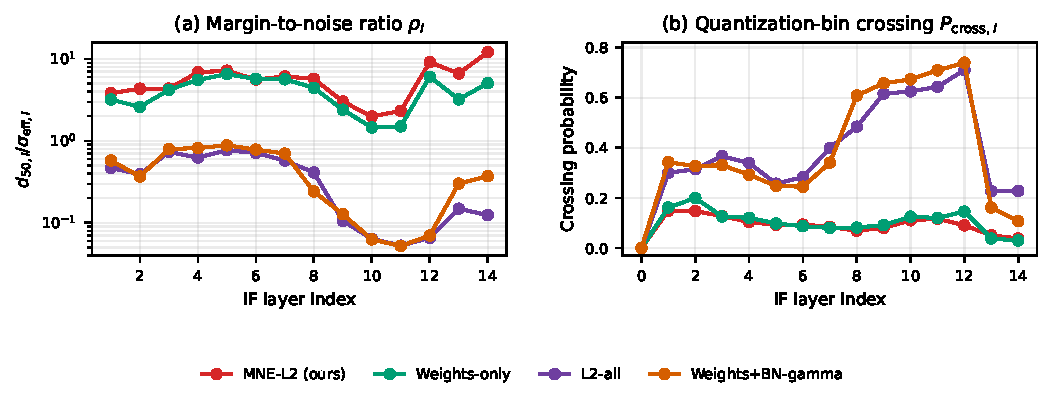
\includegraphics[width=\textwidth]{images/layerwise_diagnostics.pdf}
  \caption{Layerwise CIFAR-10 VGG16 diagnostics at fixed $\sigma=1$. All-parameter L2 and weights+BN-$\gamma$ checkpoints develop small margin-to-noise ratios and high bin-crossing probability in later blocks.}
  \label{fig:layerwise}
\end{figure}
\FloatBarrier

\section{Additional Experimental Details}

The CIFAR VGG16 source ANNs are trained for 300 epochs with batch size 128 and five independent seeds where multi-seed results are reported. Training uses SGD with momentum $0.9$, initial learning rate $0.1$, and cosine annealing. Random crops with four-pixel padding, horizontal flips, CIFAR AutoAugment, and Cutout are used during training; evaluation uses only dataset-specific normalization. MNE-L2 uses coefficient $10^{-4}$ with detached BN affine/statistical factors and detached IF thresholds. All-parameter L2 uses weight decay $5\times10^{-4}$, weights-only L1 uses $10^{-5}$, and the selective L2 scope controls use coefficient $2.5\times10^{-4}$. The scope comparison reuses single-seed CIFAR-10 checkpoints and the same evaluation protocol at every severity.

The ImageNet ResNet-18 source ANNs are trained at $T=0$ for 90 epochs with a single seed, batch size 256, SGD momentum $0.9$, initial learning rate $0.1$, and cosine annealing. Training applies a random $224\times224$ resized crop and horizontal flip; validation resizes to 256 pixels and takes a $224\times224$ center crop. Both splits use standard ImageNet normalization. The highest clean validation-accuracy checkpoint is converted with $L=T=16$ and evaluated on the 50,000-image validation split. All-parameter and weights-only L2 use coefficient $10^{-4}$, MNE-L2 uses $10^{-4}$, and weights-only L1 uses $10^{-5}$. No coefficient sweep or clean-accuracy matching was performed for the reported ImageNet comparison, and coefficients were not selected from the noisy evaluation curves.

For the CIFAR arithmetic estimate, dense ANN energy and event-driven SNN energy are
\begin{equation}
E_{\mathrm{ANN}}=N_{\mathrm{MAC}}E_{\mathrm{MAC}},\qquad
E_{\mathrm{SNN}}=T N_{\mathrm{MAC}}^{(1)}E_{\mathrm{MAC}}+N_{\mathrm{AC}}^{(>1)}E_{\mathrm{AC}},
\label{eq:energy}
\end{equation}
with $E_{\mathrm{MAC}}=4.6$ pJ and $E_{\mathrm{AC}}=0.9$ pJ. The first convolution receives analog pixels at every timestep; all later convolutional and linear layers use measured presynaptic events. Only clean ($\sigma=0$) activity is used in this estimate.

\subsection{Full CIFAR robustness and energy statistics}
\label{app:cifar-tables}

Table~\ref{tab:cifar-sigma-one} reports the full $\sigma=1$ timestep sweep for the main comparison. Tables~\ref{tab:cifar-accuracy-full} and~\ref{tab:cifar-energy-full} report clean accuracy and energy at every timestep; Table~\ref{tab:cifar-activity-full} adds per-sample activity distributions and the L2-wo/L1 controls at $T=16$. The main-paper Table~\ref{tab:cifar-deployment-main} reports the four-method $\sigma=5$ comparison. For energy accounting, we count dense operations in the first convolution at every timestep and event-triggered ACs in all later convolutional and linear layers. Every table uses all 10,000 examples in each test set; uncertainty reflects variation across five independently trained checkpoints, not measurement noise from physical hardware.

\begin{table}[t]
\caption{Top-1 accuracy under per-timestep Gaussian noise at $\sigma=1$ (mean $\pm$ sample standard deviation across five independently trained seeds).}
\label{tab:cifar-sigma-one}
\centering
\small
\begin{tabular}{llrrr}
\toprule
Dataset & Method & $T=4$ & $T=8$ & $T=16$ \\
\midrule
CIFAR-10  & L2-all & $10.10\pm0.15$ & $11.17\pm1.18$ & $23.30\pm6.46$ \\
          & MNE-L2 (ours) & $88.97\pm0.21$ & $89.76\pm0.18$ & $90.09\pm0.10$ \\
\midrule
CIFAR-100 & L2-all & $1.56\pm0.40$ & $2.88\pm0.83$ & $14.64\pm3.16$ \\
          & MNE-L2 (ours) & $58.77\pm0.28$ & $59.27\pm0.11$ & $59.48\pm0.23$ \\
\bottomrule
\end{tabular}
\end{table}

\begin{table}[t]
\caption{Full clean SNN top-1 accuracy (mean $\pm$ sample standard deviation across five independently trained seeds).}
\label{tab:cifar-accuracy-full}
\centering
\small
\begin{tabular}{llrrr}
\toprule
Dataset & Method & $T=4$ & $T=8$ & $T=16$ \\
\midrule
CIFAR-10 & L2-all & $90.29\pm0.23$ & $90.52\pm0.14$ & $90.59\pm0.13$ \\
         & L2-wo  & $90.57\pm0.18$ & $90.96\pm0.06$ & $91.10\pm0.07$ \\
         & L1-wo  & $89.09\pm0.25$ & $89.70\pm0.30$ & $89.87\pm0.20$ \\
         & MNE-L2 (ours) & $89.93\pm0.16$ & $90.31\pm0.17$ & $90.38\pm0.14$ \\
\midrule
CIFAR-100 & L2-all & $61.83\pm0.47$ & $62.22\pm0.49$ & $62.27\pm0.37$ \\
          & L2-wo  & $62.68\pm0.54$ & $63.57\pm0.31$ & $63.83\pm0.26$ \\
          & L1-wo  & $52.37\pm0.95$ & $52.89\pm0.71$ & $53.13\pm0.73$ \\
          & MNE-L2 (ours) & $59.24\pm0.21$ & $59.62\pm0.31$ & $59.62\pm0.22$ \\
\bottomrule
\end{tabular}
\end{table}

\begin{table*}[t]
\caption{Full clean CIFAR VGG16 arithmetic-energy estimates (mean $\pm$ sample standard deviation across five independently trained seeds). ANN energy is $1.5277$ mJ on CIFAR-10 and $1.5294$ mJ on CIFAR-100. ``Ratio'' is ANN energy divided by estimated SNN energy.}
\label{tab:cifar-energy-full}
\centering
\scriptsize
\setlength{\tabcolsep}{2.2pt}
\begin{tabular}{llrrrrrr}
\toprule
& & \multicolumn{2}{c}{$T=4$} & \multicolumn{2}{c}{$T=8$} & \multicolumn{2}{c}{$T=16$} \\
Dataset & Method & Energy (mJ) & Ratio & Energy (mJ) & Ratio & Energy (mJ) & Ratio \\
\midrule
CIFAR-10 & L2-all & $0.1421\pm0.0015$ & $10.75\pm0.11$ & $0.2877\pm0.0030$ & $5.31\pm0.05$ & $0.5848\pm0.0060$ & $2.61\pm0.03$ \\
         & L2-wo  & $0.1227\pm0.0008$ & $12.45\pm0.08$ & $0.2483\pm0.0016$ & $6.15\pm0.04$ & $0.5050\pm0.0033$ & $3.03\pm0.02$ \\
         & L1-wo  & $0.0975\pm0.0010$ & $15.67\pm0.17$ & $0.1969\pm0.0022$ & $7.76\pm0.08$ & $0.4019\pm0.0046$ & $3.80\pm0.04$ \\
         & MNE-L2 (ours) & $0.1141\pm0.0005$ & $13.39\pm0.06$ & $0.2312\pm0.0012$ & $6.61\pm0.03$ & $0.4716\pm0.0026$ & $3.24\pm0.02$ \\
\midrule
CIFAR-100 & L2-all & $0.1354\pm0.0020$ & $11.30\pm0.16$ & $0.2742\pm0.0039$ & $5.58\pm0.08$ & $0.5577\pm0.0078$ & $2.74\pm0.04$ \\
          & L2-wo  & $0.1271\pm0.0005$ & $12.03\pm0.04$ & $0.2569\pm0.0010$ & $5.95\pm0.02$ & $0.5225\pm0.0021$ & $2.93\pm0.01$ \\
          & L1-wo  & $0.1043\pm0.0011$ & $14.66\pm0.16$ & $0.2109\pm0.0025$ & $7.25\pm0.09$ & $0.4294\pm0.0052$ & $3.56\pm0.04$ \\
          & MNE-L2 (ours) & $0.1197\pm0.0009$ & $12.77\pm0.10$ & $0.2424\pm0.0019$ & $6.31\pm0.05$ & $0.4942\pm0.0037$ & $3.09\pm0.02$ \\
\bottomrule
\end{tabular}
\end{table*}

\begin{table*}[t]
\caption{Clean activity distribution, clean arithmetic energy, and $\sigma=1$ robustness at $T=16$. Within each seed, firing density is the fraction of nonzero entries across all IF outputs and is summarized over 10,000 samples by its mean, median, and 95th percentile; entries report the mean $\pm$ sample standard deviation of these statistics across five independently trained seeds. Energy uses clean mean activity only.}
\label{tab:cifar-activity-full}
\centering
\scriptsize
\setlength{\tabcolsep}{2.2pt}
\begin{tabular}{llrrrrrr}
\toprule
Dataset & Method & Clean acc. (\%) & Fire mean & Fire median & Fire p95 & Energy (mJ) & Acc. at $\sigma=1$ (\%) \\
\midrule
CIFAR-10 & L2-all          & $90.59\pm0.13$ & $0.105\pm0.003$ & $0.105\pm0.003$ & $0.120\pm0.004$ & $0.585\pm0.006$ & $23.30\pm6.46$ \\
         & \textbf{MNE-L2 (ours)} & $90.38\pm0.14$ & $0.083\pm0.001$ & $0.083\pm0.001$ & $0.099\pm0.002$ & $0.472\pm0.003$ & $90.09\pm0.10$ \\
         & L2-wo           & $91.10\pm0.07$ & $0.102\pm0.001$ & $0.103\pm0.001$ & $0.118\pm0.001$ & $0.505\pm0.003$ & $90.82\pm0.11$ \\
         & L1-wo           & $89.87\pm0.20$ & $0.077\pm0.001$ & $0.077\pm0.001$ & $0.090\pm0.002$ & $0.402\pm0.005$ & $89.60\pm0.16$ \\
\midrule
CIFAR-100 & L2-all          & $62.27\pm0.37$ & $0.106\pm0.003$ & $0.106\pm0.003$ & $0.121\pm0.004$ & $0.558\pm0.008$ & $14.64\pm3.16$ \\
          & \textbf{MNE-L2 (ours)} & $59.62\pm0.22$ & $0.090\pm0.001$ & $0.090\pm0.001$ & $0.107\pm0.002$ & $0.494\pm0.004$ & $59.48\pm0.23$ \\
          & L2-wo           & $63.83\pm0.26$ & $0.105\pm0.001$ & $0.106\pm0.001$ & $0.120\pm0.001$ & $0.522\pm0.002$ & $63.79\pm0.25$ \\
          & L1-wo           & $53.13\pm0.73$ & $0.084\pm0.002$ & $0.085\pm0.002$ & $0.101\pm0.002$ & $0.429\pm0.005$ & $53.08\pm0.76$ \\
\bottomrule
\end{tabular}
\end{table*}

\FloatBarrier

\subsection{Depth transfer across VGG13 and VGG19}
\label{app:depth-transfer}

We repeat the per-timestep Gaussian-noise sweep at $L=T=16$ using VGG13 and VGG19 on CIFAR-10 and CIFAR-100. Each curve reports the mean and sample standard deviation across five independently trained seeds. In addition to the four main regularizers, this control includes Calibrated MNE with the fixed $\alpha=0.1$ configuration; $\alpha$ is a prescribed training schedule rather than a gradient-triggered or adaptive choice.

\begin{figure}[t]
  \centering
  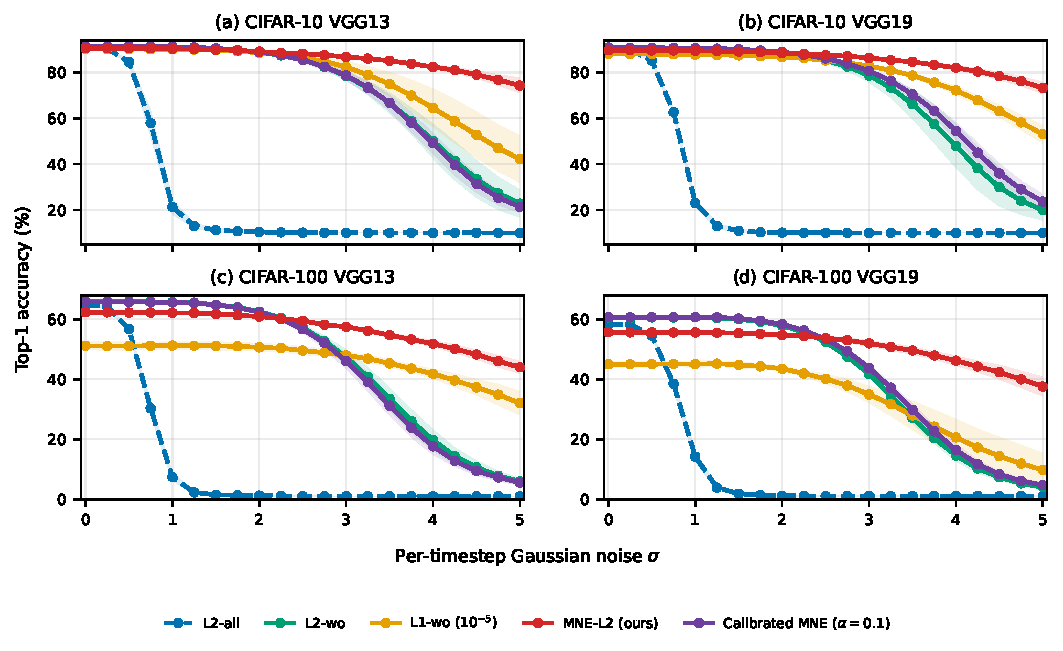
\includegraphics[width=\textwidth]{images/vgg_depth_transfer.pdf}
  \caption{Depth-transfer robustness at $L=T=16$ under Gaussian noise applied independently at each SNN timestep. Curves are five-seed means and bands show sample standard deviations. MNE-L2 is highlighted in red; Calibrated MNE is included only as an appendix control.}
  \label{fig:vgg-depth-transfer}
\end{figure}

\begin{table}[t]
\caption{Additional-depth accuracy endpoints (mean $\pm$ sample standard deviation across five independently trained seeds). The best value within each architecture, dataset, and noise condition is bold.}
\label{tab:vgg-depth-endpoints}
\centering
\scriptsize
\setlength{\tabcolsep}{3.4pt}
\begin{tabular}{llrrrr}
\toprule
& & \multicolumn{2}{c}{CIFAR-10} & \multicolumn{2}{c}{CIFAR-100} \\
Architecture & Method & $\sigma=0$ & $\sigma=5$ & $\sigma=0$ & $\sigma=5$ \\
\midrule
VGG13 & L2-all     & $90.93\pm0.14$ & $9.99\pm0.01$   & $64.73\pm0.19$ & $1.01\pm0.01$ \\
      & L2-wo      & $\mathbf{91.44\pm0.14}$ & $22.78\pm5.99$ & $\mathbf{65.94\pm0.15}$ & $5.96\pm0.96$ \\
      & L1-wo      & $90.30\pm0.14$ & $42.17\pm10.20$ & $51.16\pm1.31$ & $32.06\pm3.92$ \\
      & MNE-L2 (ours) & $90.61\pm0.19$ & $\mathbf{74.28\pm3.25}$ & $62.41\pm0.15$ & $\mathbf{44.01\pm2.02}$ \\
      & Cal. MNE   & $91.41\pm0.13$ & $21.38\pm2.58$ & $65.82\pm0.22$ & $5.59\pm0.92$ \\
\midrule
VGG19 & L2-all     & $90.19\pm0.12$ & $10.00\pm0.00$ & $58.37\pm0.64$ & $1.13\pm0.18$ \\
      & L2-wo      & $90.69\pm0.18$ & $19.95\pm4.44$ & $60.62\pm0.32$ & $4.03\pm0.65$ \\
      & L1-wo      & $88.09\pm0.25$ & $53.04\pm3.85$ & $45.04\pm1.01$ & $9.77\pm5.59$ \\
      & MNE-L2 (ours) & $89.67\pm0.06$ & $\mathbf{73.23\pm2.50}$ & $55.75\pm0.43$ & $\mathbf{37.60\pm3.19}$ \\
      & Cal. MNE   & $\mathbf{90.84\pm0.03}$ & $23.66\pm3.05$ & $\mathbf{60.73\pm0.22}$ & $4.73\pm0.76$ \\
\bottomrule
\end{tabular}
\end{table}

Across VGG13/16/19, MNE-L2 attains $74.28/72.06/73.23\%$ at $\sigma=5$ on CIFAR-10 and $44.01/41.14/37.60\%$ on CIFAR-100. Calibrated MNE closely follows L2-wo despite matching or slightly exceeding its clean accuracy, while L1-wo incurs a substantial CIFAR-100 clean-accuracy cost that grows from VGG13 to VGG19. Thus the high-noise MNE-L2 advantage transfers across the three completed depths, although the CIFAR-100 endpoint declines with depth.

\FloatBarrier

\subsection{Compact MNIST-family controls}
\label{app:compact}

We use MNIST \citep{lecun1998gradient} and Fashion-MNIST \citep{xiao2017fashion} with a 2,081-parameter CNN: two $3\times3$ convolution-BN-IF blocks with 2 and 4 channels, $2\times2$ max pooling, and a linear classifier. Source ANNs are trained for 30 epochs with five independent seeds and converted at $T\in\{4,8,16\}$. We compare MNE-L2, orthogonal weight regularization, no regularization, and optimizer L2. During the low-latency sweep, Gaussian noise is added after both the input IF and first hidden IF at $\sigma\in\{0,0.25,0.5\}$; each nonzero point averages three paired streams within each training seed.

For the compact CNN, the dense ANN baseline is 30,184 MACs per sample. The event counter charges every nonzero presynaptic activation once for each valid downstream connection. It counts both convolutional layers and the classifier, including edge effects from padding, and accumulates over all $T$ timesteps. Reported means and standard deviations are across five independently trained checkpoints.

Figure~\ref{fig:latency} gives the compact low-latency view. At $T=4$, the event-SynOps ratio ranges from 0.36 to 0.45 on Fashion-MNIST and 0.63 to 0.65 on MNIST; at $T=16$, it rises to 1.54--1.97 and 2.71--2.86. These are algorithmic operation counts rather than wall-clock latency or hardware energy \citep{davies2018loihi,horowitz2014computing}.

\begin{figure}[h!]
  \centering
  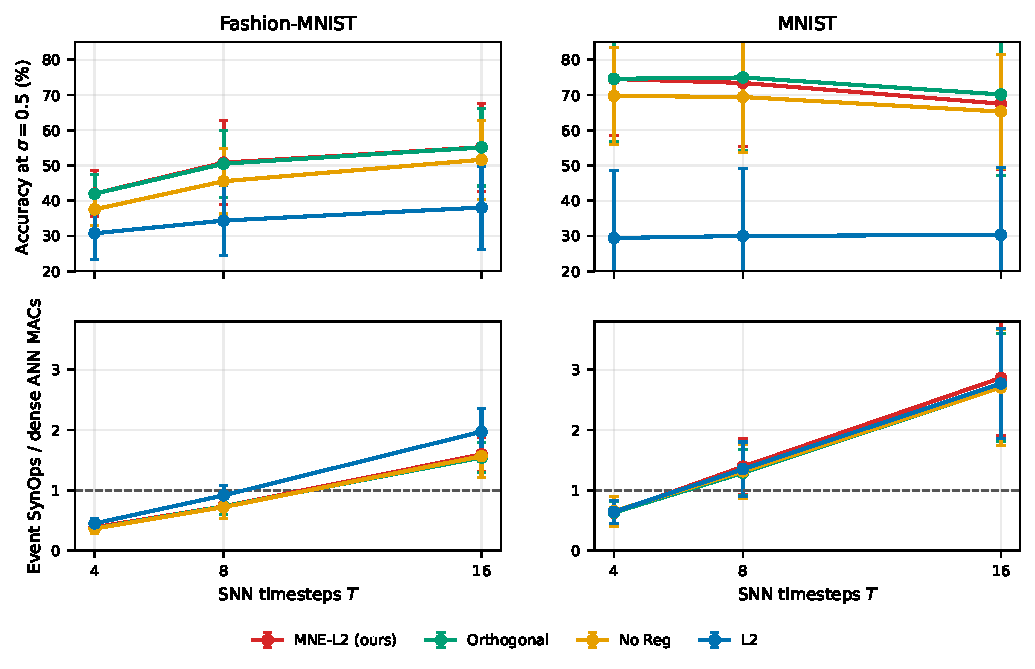
\includegraphics[width=0.82\textwidth]{images/latency_reliability_efficiency.pdf}
  \caption{Appendix compact-model control. Top: five-seed accuracy under two-site Gaussian noise with $\sigma=0.5$. Bottom: event-driven synaptic-operation proxy relative to one dense ANN MAC pass; the dashed line marks ratio 1. Error bars are standard deviations across training seeds.}
  \label{fig:latency}
\end{figure}

\begin{table}[t]
\caption{Full five-seed accuracy at $\sigma=0.5$ (mean $\pm$ standard deviation across training seeds). Noise is injected after both the input IF and first hidden IF.}
\label{tab:full-accuracy}
\centering
\small
\begin{tabular}{llrrr}
\toprule
Dataset & Method & $T=4$ & $T=8$ & $T=16$ \\
\midrule
Fashion & MNE-L2 (ours) & $42.01\pm6.48$ & $50.81\pm11.93$ & $55.19\pm12.53$ \\
Fashion & Orthogonal & $41.98\pm5.49$ & $50.50\pm9.54$  & $55.12\pm10.95$ \\
Fashion & No Reg     & $37.53\pm4.69$ & $45.53\pm9.30$  & $51.64\pm11.19$ \\
Fashion & L2         & $30.75\pm7.49$ & $34.35\pm9.95$  & $38.06\pm11.80$ \\
\midrule
MNIST & MNE-L2 (ours) & $74.55\pm16.12$ & $73.44\pm17.98$ & $67.54\pm18.60$ \\
MNIST & Orthogonal   & $74.62\pm17.89$ & $74.99\pm20.82$ & $70.17\pm22.92$ \\
MNIST & No Reg       & $69.75\pm13.68$ & $69.44\pm15.69$ & $65.31\pm16.18$ \\
MNIST & L2           & $29.41\pm19.27$ & $30.00\pm19.23$ & $30.30\pm19.07$ \\
\bottomrule
\end{tabular}
\end{table}

\FloatBarrier

\section{Reproducibility Notes}

All reported datasets use their standard public train/test splits. The evaluation code fixes the training seed separately from the perturbation seed, stores every per-seed result before aggregation, and reports sample standard deviation rather than standard error. Figures~\ref{fig:bn-scope}, \ref{fig:robustness-benchmarks}, and~\ref{fig:vgg-depth-transfer} are generated directly from stored CSV summaries by a deterministic plotting script; curve values are neither redrawn nor transcribed. The compact event-count control uses CPU inference and 1,024 examples per checkpoint. The CIFAR activity evaluation uses each full 10,000-example test set: sample mean, median, and p95 are computed within each seed, then summarized across five independently trained seeds by mean and sample standard deviation. Only $\sigma=0$ activity enters energy; $\sigma=1$ activity is retained as a diagnostic and excluded from deployment estimates. Full VGG and ResNet training requires GPU compute; evaluation does not update model parameters.

\input{checklist.tex}

\end{document}
